\documentclass[../main.tex]{subfile}
\graphicspath{{\subfix{../images}}}
\begin{document}

% \begin{figure}[htb]
%     \centering
%     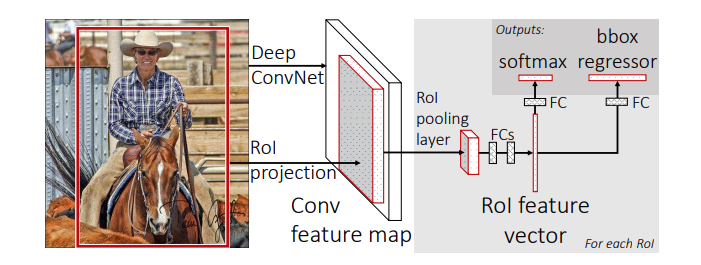
\includegraphics[width=\textwidth]{fig1.png}
%     \caption{\textbf{SSD框架。}(a) SSD 在训练期间只需要每个对象的输入图像和ground truth框。 以卷积方式,我们在不同尺寸的几个特征图中(例如(b)和(c)中的$ 8 \times  8 $和$ 4 \times  4$)的每个位置评估一小组(例如 4 个)不同长宽比的默认框。 对于每个默认框,我们预测形状偏移和所有物体类别($\left( c_1, c_2, \ldots, c_p \right)$)的置信度。 在训练时,我们首先将这些默认框与ground truth框匹配。 例如,我们将两个默认框与猫匹配,一个与狗匹配,将它们视为正例,其余视为负例。 模型损失是定位损失(例如 Smooth L1 \cite{fast})和置信度损失(例如 Softmax)的加权和。}
%     \label{fig:fig1}
% \end{figure}

\end{document}